\documentclass[a4paper,12pt]{article} % добавить leqno в [] для нумерации слева
\usepackage[a4paper,top=1.3cm,bottom=2cm,left=1.5cm,right=1.5cm,marginparwidth=0.75cm]{geometry}
%%% Работа с русским языком
\usepackage{cmap}					% поиск в PDF
\usepackage[warn]{mathtext} 		% русские буквы в фомулах
\usepackage[T2A]{fontenc}			% кодировка
\usepackage[utf8]{inputenc}			% кодировка исходного текста
\usepackage[english,russian]{babel}	% локализация и переносы
\usepackage{physics}
\usepackage{multirow}

%%% Нормальное размещение таблиц (писать [H] в окружении таблицы)
\usepackage{float}
\restylefloat{table}


\usepackage{graphicx}

\usepackage{wrapfig}
\usepackage{tabularx}

\usepackage{hyperref}
\usepackage[rgb]{xcolor}
\hypersetup{
	colorlinks=true,urlcolor=blue
}

%%% Дополнительная работа с математикой
\usepackage{amsmath,amsfonts,amssymb,amsthm,mathtools} % AMS
\usepackage{icomma} % "Умная" запятая: $0,2$ --- число, $0, 2$ --- перечисление

%% Номера формул
%\mathtoolsset{showonlyrefs=true} % Показывать номера только у тех формул, на которые есть \eqref{} в тексте.

%% Шрифты
\usepackage{euscript}	 % Шрифт Евклид
\usepackage{mathrsfs} % Красивый матшрифт
\usepackage{pgfplots}
\pgfplotsset{compat=1.9}

%% Свои команды
\DeclareMathOperator{\sgn}{\mathop{sgn}}

%% Перенос знаков в формулах (по Львовскому)
\newcommand*{\hm}[1]{#1\nobreak\discretionary{}
	{\hbox{$\mathsurround=0pt #1$}}{}}

\date{\today}

\begin{document}

\begin{titlepage}
	\begin{center}
		{\large МОСКОВСКИЙ ФИЗИКО-ТЕХНИЧЕСКИЙ ИНСТИТУТ (НАЦИОНАЛЬНЫЙ ИССЛЕДОВАТЕЛЬСКИЙ УНИВЕРСИТЕТ)}
	\end{center}
	
	\vspace{4.5cm}
	{\huge
		\begin{center}
			{\bf Отчёт о выполнении лабораторной работы 3.2.2}\\
			Резонанс напряжений в последовательном контуре
		\end{center}
	}
	\vspace{2cm}
	\begin{flushright}
		{\LARGE Автор:\\ Клименко Виталий Евгеньевич \\
			\vspace{0.2cm}
			Б01-202}
	\end{flushright}
	\vspace{8cm}
	\begin{center}
		Долгопрудный\\
		\today
	\end{center}
\end{titlepage}


\section{Введение}

 \ \ \ \textbf{Цель работы:} изучение последовательной цепи переменного тока, наблюдение резонанса напряжений.

\textbf{В работе используются:} регулировочный автотрансформатор, катушка индуктивности с выдвижным сердечником, магазин ёмкостей, реостат, резистор, амперметр, три вольтметра, ваттметр, осциллограф, универсальный мост.

\section{Теоретические сведения}

Рассмотрим электрическую цепь, состоящую из резистора $ R $ и катушки индуктивности $ L $ с импедансом $ Z_L = r_L + i \Omega L $, последовательно подключённых к внешнему источнику, ЭДС которого меняется по синусоидальному закону с частотой $ \Omega $ (рис. \ref{fig:image1}).
\begin{figure}[h]
	\center{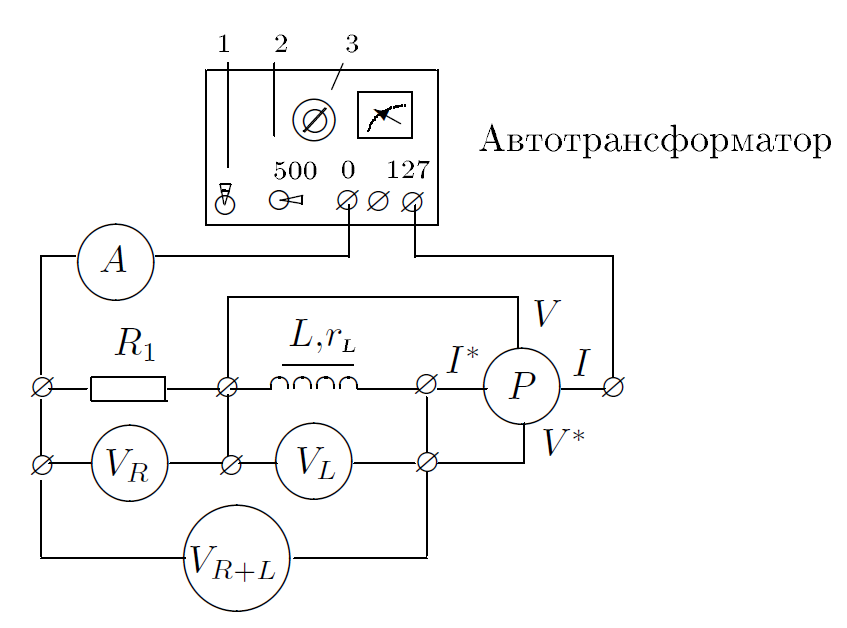
\includegraphics[scale=0.8]{Screenshot_2.png}}
	\caption{\centering Схема установки для изучения закона Ома в цепи переменного тока.}
	\label{fig:image1}
\end{figure}

Обозначим через $ U_R $ напряжение на резисторе, через $ U_L $ -- напряжение на катушке и через $ U_{R+L} $ — суммарное напряжение на катушке и на резисторе. Для этих напряжений справедливы комплексные соотношения:
\begin{equation}\label{eq:1}
{\widehat U_R} = \widehat IR, \quad {\widehat U_L} = \widehat I\left( {{r_L} + i\Omega L} \right), \quad {\widehat U_{R + L}} = \widehat I\left( {R + {r_L} + i\Omega L} \right).
\end{equation}
Напомним, что здесь $ r_L $ -- активное сопротивление катушки, которое характеризует суммарные потери энергии в катушке, в том числе потери в её ферромагнитном сердечнике.

Переходя к модулям и фазам токов и напряжений, найдём из (\ref{eq:1}):
\begin{equation}\label{eq:2}
{U_R} = I \cdot R, \quad \tg{\psi _1} = 0;
\end{equation}
\begin{equation}\label{eq:3}
{U_L} = I \cdot \sqrt {r_L^2 + {{\left( {\Omega L} \right)}^2}}, \quad \tg{\psi _2} = \frac{{\Omega L}}{{{r_L}}};
\end{equation}
\begin{equation}\label{eq:4}
{U_{R + L}} = I\sqrt {{{\left( {R + {r_L}} \right)}^2} + {{\left( {\Omega L} \right)}^2}}, \quad \tg{\psi _3} = \frac{{\Omega L}}{{R + {r_L}}}.
\end{equation}
В этих формулах $ U $ и $ I $ обозначают \textit{эффективные} значения напряжений и токов (показания приборов), как принято в электротехнике.

Измеряя с помощью трёх вольтметров значения $ U_R $, $ U_L $ и $ U_{R+L} $ и зная сопротивление резистора $ R $, нетрудно вычислить, пользуясь формулами (\ref{eq:2}), (\ref{eq:3}) и (\ref{eq:4}), силу тока в цепи, активное сопротивление катушки $ r_L $, её индуктивность $ L $, мощность $ P_L $, выделяемую на катушке, и сдвиг фаз между током и напряжением на катушке.

Рассчитаем мощность переменного тока, выделяемую в катушке. Мгновенное значение мощности равно
\begin{equation*}
P = U\left( t \right) \cdot I\left( t \right).
\end{equation*}
Средняя мощность за период $ T $ определяется формулой
\begin{equation*}
\overline P  = \frac{1}{T}\int\limits_0^T {U\left( t \right) \cdot I\left( t \right)dt}.
\end{equation*}
Полагая $ \displaystyle I\left( t \right) = I\sqrt 2 \cos \Omega t $, $ U\left( t \right) = U\sqrt 2 \cos \left( {\Omega t + \psi } \right) $, получим после интегрирования:
\begin{equation}\label{eq:5}
{P_L} = {U_L} \cdot I\cos \psi  = {I^2} \cdot {r_L}.
\end{equation}
Средняя мощность, выделяющаяся в катушке самоиндукции, определяется, таким образом, действительной частью её импеданса.

Активное сопротивление катушки $ r_L $ можно определить, если включить её в последовательный колебательный контур с известными параметрами -- сопротивлением $ R $ и ёмкостью $ C $ (рис. \ref{fig:image2}). В контуре, настроенном в резонанс на частоту $ \Omega $ внешнего источника (собственная частота контура и внешняя совпадают: $ \omega_0 = \Omega $, реактивные сопротивления индуктивности и ёмкости одинаковы:
\begin{equation}\label{eq:6}
{\omega _0}L = \frac{1}{{{\omega _0}C}}.
\end{equation}
Определив каким-либо экспериментальным способом добротность $ Q $ этого контура, можно рассчитать полное сопротивление контура $ R_{\Sigma} $ в резонансе, поскольку
\begin{equation}\label{eq:7}
Q = \frac{{{\omega _0}L}}{{{R_\Sigma }}} = \frac{1}{{{\omega _0}C{R_\Sigma }}}.
\end{equation}
Резонансное сопротивление контура $ R_{\Sigma} $, включает в себя известное со противление резистора $ R $ и активное сопротивление катушки $ r_L $:
\begin{equation}\label{eq:8}
{R_\Sigma } = R + {r_L}.
\end{equation}

\section{Экспериментальная установка}
Схема установки для исследования закона Ома в цепи переменного тока представлена на рис. \ref{fig:image1}. Цепь, состоящая из резистора $ R_1 \simeq 100 $ Ом и катушки $ L $ с выдвижным сердечником, подключена к автотрансформатору, выходное напряжение которого можно менять от $ 0 $ до $ 127 $ В. Напряжения на каждом из элементов и суммарное напряжение цепи измеряются тремя вольтметрами: $ V_R $, $ V_L $ и $ V_{R+L} $. Амперметр $ A $ измеряет ток в цени, а ваттметр $ P $ -- мощность, выделяющуюся на катушке.

Ваттметр электродинамической системы состоит из двух катушек, одна из которых вращается в магнитном поле другой, если через них течёт ток. Токовая катушка ваттметра $ II $* включается последовательно в исследуемую цепь, а катушка напряжений (потенциальная) $ VV $* -- параллельно к элементу, в котором измеряется выделяемая мощность.

Два из четырёх зажимов ваттметра помечены звёздочкой (*). Эти зажимы надо соединить вместе. Предел измерений устанавливается при помощи переключателей или штепселей, которые вставляются в соответствующие гнёзда: произведение цифр против штепселя токовой катушки $ II $* и против переключателя катушки напряжений $ VV $* определяет мощность, соответствующую отклонению стрелки на всю шкалу. Отсчёт мощности ведётся но любой из шкал, обозначенных буквой $ P $.

\begin{figure}[h]
	\center{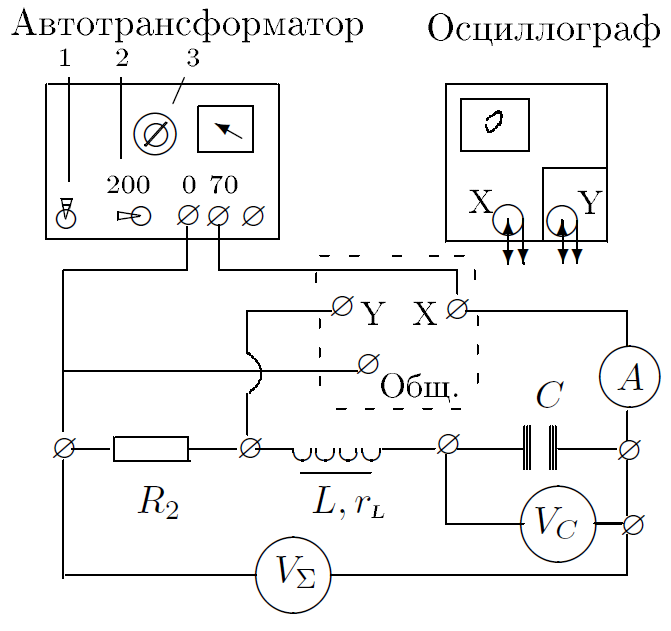
\includegraphics[scale=0.8]{Screenshot_3.png}}
	\caption{\centering Схема установки для наблюдения резонанса напряжений.}
	\label{fig:image2}
\end{figure}

Схема установки для изучения резонанса напряжений изображена на рис. \ref{fig:image2}. Последовательно соединены резистор $ R_2 \approx 5 $ Ом, катушка $ L $ и магазин ёмкостей $ C $. Амперметр $ A $ измеряет ток в цепи, вольтметр $ V_C $ — напряжение на ёмкости, вольтметр $ V_{\Sigma} $ -- суммарное напряжение на контуре. Резонанс можно зафиксировать с помощью осциллографа, если подать на вход $ X $ напряжение с контура, а на вход $ Y $ -- напряжение с резистора $ R_2 $, пропорциональное току в цепи. В общем случае на экране виден эллипс. При резонансе эллипс вырождается в прямую линию.
Резонансные напряжения на контуре $ U_{\Sigma,\text{ рез}} $ и на ёмкости $ U_{C,\text{ рез}} $ равны соответственно
\begin{equation}\label{eq:9}
U_{\Sigma,\text{ рез}} = I_{\text{рез}}R_{\Sigma}, \quad U_{C,\text{ рез}} = \dfrac{I_{\text{рез}}}{\Omega C}.
\end{equation}
Сравнивая (\ref{eq:7}) и (\ref{eq:9}), получим
\begin{equation}\label{eq:10}
Q = \dfrac{U_{C,\text{ рез}}}{U_{\Sigma,\text{ рез}}}, \quad {\sigma _Q} = Q\sqrt {{{\left( {\frac{{{\sigma_{U_{C,\text{ рез}}}}}}{U_{C,\text{ рез}}}} \right)}^2} + {{\left( {\frac{{{\sigma_{U_{\Sigma,\text{ рез}}}}}}{U_{\Sigma,\text{ рез}}}} \right)}^2}} .
\end{equation}
Формула (\ref{eq:10}) показывает, что добротность контура может быть найдена по измеренным значениям напряжений на контуре и на конденсаторе при резонансе. Зная добротность контура и ёмкость $ C $, можно рассчитать $ R_{\Sigma} $, по формуле (\ref{eq:7}), а затем определить $ r_L $.
\section{Обработка и предоставление результатов}
\begin{table}[H]
\centering
\resizebox{500pt}{!}{
\begin{tabular}{|r|r|r|r|r|r|r|r|r|r|r|r|}
\hline
\multicolumn{1}{|c|}{N} &
  \multicolumn{1}{c|}{C\_n, nF} &
  \multicolumn{1}{c|}{f\_0n, kHz} &
  \multicolumn{1}{c|}{U(f\_0n), V} &
  \multicolumn{1}{c|}{E(f\_0n), V} &
  \multicolumn{1}{c|}{L, muH} &
  \multicolumn{1}{c|}{rho, Om} &
  \multicolumn{1}{c|}{Z\_res, Om} &
  \multicolumn{1}{c|}{Q} &
  \multicolumn{1}{c|}{R\_sum, Ом} &
  \multicolumn{1}{c|}{R\_sm, Ом} &
  \multicolumn{1}{c|}{R\_L, Ом} \\ \hline
1                                             & 25,1                  & 32   & 1,5  & 0,3019 & 986,523 & 198,252 & 5008,28 & 25,2751 & 7,839786 & 0,19825 & 4,141534 \\ \hline
2                                             & 33,2                  & 27,8 & 1,38 & 0,302  & 988,219 & 172,527 & 4606,09 & 26,7113 & 6,455678 & 0,17253 & 2,78315  \\ \hline
3                                             & 47,3                  & 23   & 0,99 & 0,3021 & 1013,36 & 146,37  & 3303,28 & 22,5795 & 6,479139 & 0,14637 & 2,832769 \\ \hline
4                                             & 57,4                  & 21   & 0,85 & 0,3021 & 1001,68 & 132,102 & 2836,15 & 21,4803 & 6,146801 & 0,1321  & 2,514699 \\ \hline
5                                             & 67,5                  & 19,4 & 0,7  & 0,302  & 998,099 & 121,6   & 2336,42 & 19,2237 & 6,322337 & 0,1216  & 2,700736 \\ \hline
6                                             & 82,7                  & 17,7 & 0,59 & 0,302  & 978,653 & 108,783 & 1969,27 & 18,1119 & 6,003121 & 0,10878 & 2,394338 \\ \hline
7                                             & 101,6                 & 16,1 & 0,48 & 0,3019 & 962,798 & 97,3466 & 1602,65 & 16,4717 & 5,906938 & 0,09735 & 2,309592 \\ \hline
                                              &                       &      &      &        &         &         &         &         &          &         &          \\ \hline
\multicolumn{1}{|l|}{Ср. знач.}        & \multicolumn{1}{l|}{} &      &      &        & 989,905 &         &         &         &          &         & 2,810974 \\ \hline
\multicolumn{1}{|l|}{Случ. погр.} & \multicolumn{1}{l|}{} &      &      &        & 16,4908 &         &         &         &          &         & 0,618673 \\ \hline
\end{tabular}
}
\end{table}
\end{document}